\section*{Ziel}
    Mit diesem Versuch sollen die Eigenschaften von Mikrowellen in einem Hohlleiter untersucht werden.
    Außerdem soll sich mit dem zur Erzeugung der Mikrowellen verwendete Reflexklystron vertraut gemacht werden.
\section{Theorie}
    \label{sec:theorie}
    \subsection{Mikrowellen}
    \label{sec:mikrowellen}
        Mikrowellen sind elektromagnetische Wellen im Frequenzbereich von \num{1} bis \SI{300}{\giga\hertz} und haben dementsprechend eine Wellenlänge von \SI{30}{\centi\metre} bis \SI{1}{\milli\metre}.
        Durch die entsprechende Wellenlänge sind Mikrowellen perfekt geeignet, um Dipolschwingungen in Wasser anzuregen und werden daher in den Mikrowellenherden verwendet.
        Außerdem sind Mikrowellen vor allem in der Kommunikationstechnik in vielen Bereichen in Benutzung.
    \subsection{Reflexklystron}
    \label{sec:Reflexklystron}
        Ein Reflexklystron ist eine spezielle Art eines Klystrons, welches hier verwendet wird, um die Mikrowellen zu erzeugen.
        Der grobe Aufbau des Reflexklystrons ist in Abbildung \ref{fig:reflexklystron} zu sehen.
        \begin{figure}
            \centering
            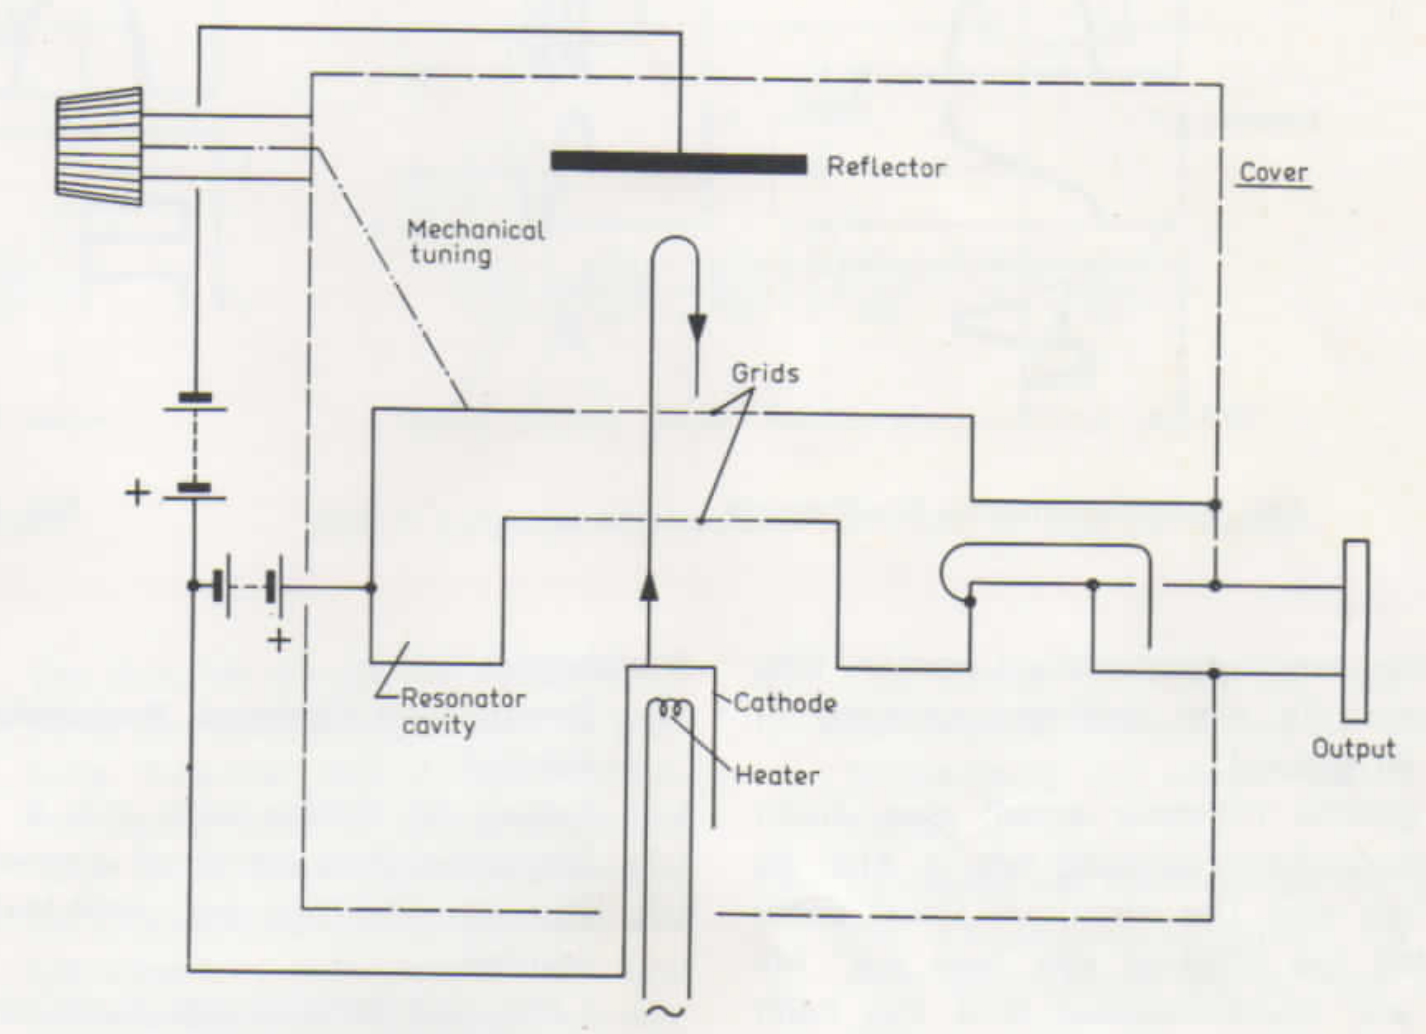
\includegraphics[width = 0.75\textwidth]{bilder/Reflexklystron.png}
            \caption{Der Aufbau eines Reflexklystrons.}
            \label{fig:reflexklystron}
        \end{figure}
        Das Klystron besteht aus einer Heiz-Kathode die Elektronen emittiert, von der Heiz-Kathode aus werden die Elektronen mit einer Anode in Richtung eines Gitters beschleunigt.
        Das Gitter ist eine Teil eines Torus-Hohlraumresonators für hohe Frequenzen in dem eine Geschwindigkeitsmodulation der Elektronen stattfindet, wenn diese durch die Gitterwände laufen.
        Elektronen, die früh in den Hohlraumresonator gelangen werden weiter beschleunigt, wohingegen Elektronen, die spät in den Resonator gelangen verlangsamt werden. Nach dem Resonator treffen alle Elektronen auf einen Reflektor und passieren erneut den Resonator.
        Mit richtiger Einstellung der Reflektorspannung ist es möglich, dass dabei alle Elektronen gleichzeitig den Resonator erreichen.
        Beim Durchlaufen des Resonators werden die Elektronen nun abgebremst und geben ihre Energie an den Schwingkreis ab. Die maximale Abbremsung findet immer bei $(n + \frac{3}{4})$ der Periodendauer des Resonators statt.
        Wird die Reflektorspannung nun durchlaufen, ergibt sich der Zusammenhang von Frequenz und Output, wie er in Abbildung \ref{fig:frequenzmodulation} zu sehen ist.
        \begin{figure}
            \centering
            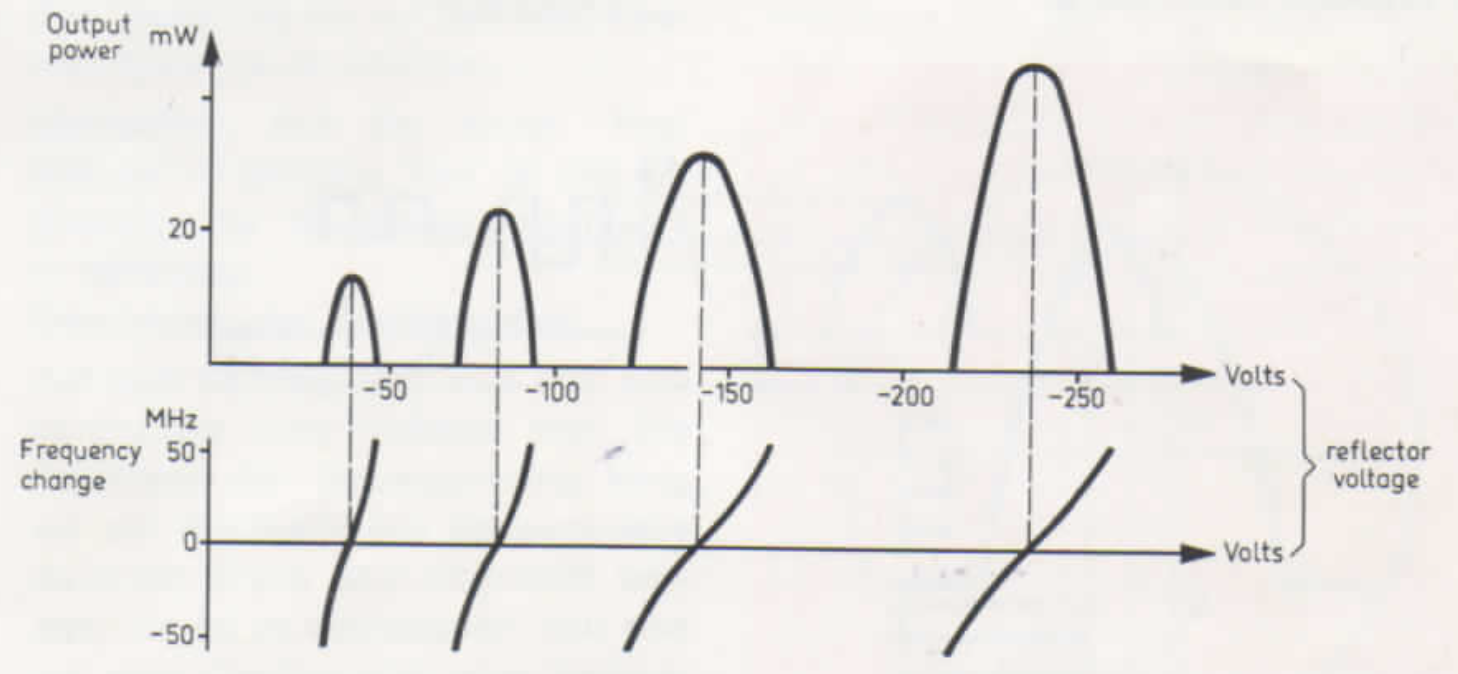
\includegraphics[width = 0.75\textwidth]{bilder/Frequenzmodulation.png}
            \caption{Frequenzmodulation}
            \label{fig:frequenzmodulation}
        \end{figure}
    \subsection{Mikrowellen in einem Hohlleiter}
    \label{sec:Hohlleiter}
        In diesem Versuch werden die erzeugten Mikrowellen innerhalb eines Hohlleiters transmittiert.
        In einem idealen unendlich ausgedehnten Hohlleiter oder einem Hohlleiter der mit einem Wiederstand abgeschlossen ist, treten dabei keine Reflexionen auf.
        Bei Unstetigkeiten im Hohlleiter wird die EM-Welle allerdings reflektiert. 
        Die Feldstärke der neuen Welle ergibt sich durch Addition der Amplituden der reflektierten und einlaufenden Wellen.
        Durch diese Addition können sich stehende Wellen im Leiter ausbilden, deren Wellenlänge über den halben Abstand zwischen zwei Maxima oder Minima bestimmt werden kann.
        Für einen Hohlleiter, der mit Luft gefüllt ist, ergibt sich:
        \begin{equation}
            \lambda_g = \frac{\lambda_0}{\sqrt{1-\left(\frac{\lambda_0}{\lambda_c}\right)^2}}
        \end{equation}
        wobei $\lambda_0$ die Wellenlänge im Vakuum und $\lambda_c = 2a$ die kritische Wellenlänge für eine Halbwellen-Änderung in eine Richtung eines rechteckigen Hohlleiters der Breite $a$ ist.
        Dadurch ergibt sich für die Frequenz:
        \begin{equation}
            \label{eqn:frequenz}
            f = \frac{c}{\lambda_0} = c \cdot \sqrt{\left(\frac{1}{\lambda_g}\right)^2 + \left(\frac{1}{2a}\right)^2}
        \end{equation}
        Das Stehwellenverhältnis bzw. die Welligkeit $S$ ist das Verhältnis von maximaler und minimaler Feldstärke im Hohlleiter.
        \begin{equation}
            S = \frac{E_{max}}{E_{min}}
        \end{equation}